\documentclass[
	% -- opções da classe memoir --
	12pt,				% tamanho da fonte
	openright,			% capítulos começam em pág ímpar (insere página vazia caso preciso)
	%twoside,			% para impressão em verso e anverso. Oposto a oneside
	oneside,
	a4paper,			% tamanho do papel. 
	% -- opções da classe abntex2 --
	%chapter=TITLE,		% títulos de capítulos convertidos em letras maiúsculas
	%section=TITLE,		% títulos de seções convertidos em letras maiúsculas
	%subsection=TITLE,	% títulos de subseções convertidos em letras maiúsculas
	%subsubsection=TITLE,% títulos de subsubseções convertidos em letras maiúsculas
	% -- opções do pacote babel --
	english,			% idioma adicional para hifenização
	french,				% idioma adicional para hifenização
	spanish,			% idioma adicional para hifenização
	brazil				% o último idioma é o principal do documento
	]{abntex2}

% ---
% Pacotes básicos 
% ---
\usepackage{lmodern}			% Usa a fonte Latin Modern			
\usepackage[T1]{fontenc}		% Selecao de codigos de fonte.
\usepackage[utf8]{inputenc}		% Codificacao do documento (conversão automática dos acentos)
\usepackage{lastpage}			% Usado pela Ficha catalográfica
\usepackage{xcolor}
\usepackage{tabu}
\usepackage{float}
\usepackage{colortbl}
\usepackage{enumitem}
\usepackage{indentfirst}		% Indenta o primeiro parágrafo de cada seção.
\usepackage{color}				% Controle das cores
\usepackage{graphicx}			% Inclusão de gráficos
\usepackage{microtype} 			% para melhorias de justificação
\usepackage{minted}
\usepackage{hyperref}
\usepackage{listings}

% ---
		
% ---
% Pacotes adicionais, usados apenas no âmbito do Modelo Canônico do abnteX2
% ---
\usepackage{lipsum}				% para geração de dummy text
% ---

% ---
% Pacotes de citações
% ---
\usepackage[brazilian,hyperpageref]{backref}	 % Paginas com as citações na bibl
\usepackage[alf]{abntex2cite}	% Citações padrão ABNT
% --- 
% CONFIGURAÇÕES DE PACOTES
% --- 
% ---
% Configurações do pacote backref
% Usado sem a opção hyperpageref de backref
\renewcommand{\backrefpagesname}{Citado na(s) página(s):~}
% Texto padrão antes do número das páginas
\renewcommand{\backref}{}
% Define os textos da citação
\renewcommand*{\backrefalt}[4]{
	\ifcase #1 %
		Nenhuma citação no texto.%
	\or
		Citado na página #2.%
	\else
		Citado #1 vezes nas páginas #2.%
	\fi}%
% ---

% ---
% Informações de dados para CAPA e FOLHA DE ROSTO
% ---
\title{Classificação de Músicas de acordo com a emoção utilizando Inteligência Artificial}
\autor{Gabriel Hideki e Gabriel Lins}
\local{São Paulo -- Brasil}
\data{2019}
\orientador{Adalberto Bosco Castro Pereira}
%\coorientador{Nome Completo}
\instituicao{%
  Centro Universitário Senac - Santo Amaro
  \par
  Bacharelado em Ciência da Computação
}
\tipotrabalho{Monografia (Graduação)}
% O preambulo deve conter o tipo do trabalho, o objetivo, 
% o nome da instituição e a área de concentração 
\preambulo{Monografia apresentada na disciplina Trabalho de Conclusão de Curso, como parte dos requisitos para obtenção do título de Bacharel em Ciência da Computação.}
% ---

% ---
% Configurações de aparência do PDF final
\addto{\captionsbrazil}{\renewcommand{\bibname}{Refer\^{e}ncias}}
% alterando o aspecto da cor azul
\definecolor{blue}{RGB}{41,5,195}

% informações do PDF
\makeatletter

\lstset{frame=tb,
  language=c,
  aboveskip=3mm,
  belowskip=3mm,
  showstringspaces=false,
  columns=flexible,
  basicstyle={\small\ttfamily},
  numbers=none,
  numberstyle=\tiny\color{gray},
  keywordstyle=\color{blue},
  commentstyle=\color{dkgreen},
  stringstyle=\color{mauve},
  breaklines=true,
  breakatwhitespace=true,
  tabsize=3
}


\hypersetup{
     	%pagebackref=true,
		pdftitle={\@title}, 
		pdfauthor={\@author},
    	pdfsubject={\imprimirpreambulo},
	    pdfcreator={LaTeX with abnTeX2},
		pdfkeywords={abnt}{latex}{abntex}{abntex2}{trabalho acadêmico}, 
		colorlinks=true,       		% false: boxed links; true: colored links
    	linkcolor=black,          	% color of internal links
    	citecolor=black,        		% color of links to bibliography
    	filecolor=magenta,      		% color of file links
		urlcolor=blue,
		bookmarksdepth=4
}
\makeatother
% --- 

% --- 
% Espaçamentos entre linhas e parágrafos 
% --- 

% O tamanho do parágrafo é dado por:
\setlength{\parindent}{1.3cm}

% Controle do espaçamento entre um parágrafo e outro:
\setlength{\parskip}{0.2cm}  % tente também \onelineskip

% ---
% compila o indice
% ---
\makeindex
% ---

% ----
% Início do documento
% ----
\begin{document}

% Retira espaço extra obsoleto entre as frases.
\frenchspacing 

% ----------------------------------------------------------
% ELEMENTOS PRÉ-TEXTUAIS
% ----------------------------------------------------------
% \pretextual

% ---
% Capa
% ---
\imprimircapa
\imprimirfolhaderosto
%*
% ---

% ---
% RESUMOS
% ---

\setlength{\absparsep}{18pt}
\begin{resumo}
  
\noindent 
%RESUMO EM PT-BR
Com o crescimento do consumo de mídias audiovisuais, houve um aumento no interesse em retornar essas mídias de maneira mais eficiente. Música é uma mídia que esta diretamente ligada as emoções, e automatizar tal classificação facilitaria o acesso e aumentaria a qualidade com a qual essa informação é entregue. Esse trabalho descreve técnicas para classificar músicas em relação às suas emoções causadas, através de suas informações técnicas e letras, utilizando a técnica de KNN e redes neurais. 

\noindent \textbf{Palavras-chaves}: Reconhecimento de emoções em músicas, KNN, Aprendizado de máquina.

\end{resumo}
{
\setlength{\absparsep}{18pt}
\selectlanguage{english}
\begin{resumo}
%RESUMO EM EN

With the growth in consuming of audiovisual media, there was an increase in the interest of returning these media more efficiently. Music is a media that is directly linked to emotions, and automating such classification would facilitate access and increase the quality with which that information is delivered. This work describes techniques for classifying songs in relation to their caused emotions, through their technical information and lyrics, using the KNN technique and neural networks.

\noindent \textbf{Palavras-chaves}: Music Emotion Recognition, KNN, Machine Learning.
\end{resumo}
}

% ---
% inserir lista de tabelas
% ---
\pdfbookmark[0]{\listtablename}{lot}
% \listoftables*
\cleardoublepage
% ---

% ---
% inserir lista de abreviaturas e siglas
% ---
\begin{siglas}
  \item[API] Application Programming Interface
  \item[CNN] Convolutional Neural Network (Rede Neural Convolucional)
  \item[IA] Inteligência Artificial
  \item[KNN] K-Nearest Neighbors
  \item[MLP] Multilayer Perceptron
  \item[NN] Neural Network (Rede Neural)
  \item[TCLE] Termo de Consentimento Livre e Esclarecido
  \item[TF-IDF] Term Frequency-Inverse Document Frequency
\end{siglas}
% ---

% ---
% inserir o sumario
% ---
\pdfbookmark[0]{\contentsname}{toc}
\tableofcontents*
\cleardoublepage
% ---


\renewcommand{\listfigurename}{Lista de Figuras}
\pdfbookmark[1]{\contentsname}{fig}
\listoffigures
\cleardoublepage

% ----------------------------------------------------------
% ELEMENTOS TEXTUAIS
% ----------------------------------------------------------
\textual

% ----------------------------------------------------------
% Capitulo 1
% ----------------------------------------------------------
\chapter[Introdução]{Introdução}
%texto de referencia

%https://www.researchgate.net/publication/254004106_Machine_Recognition_of_Music_Emotion_A_Review/download

%http://citeseerx.ist.psu.edu/viewdoc/download?doi=10.1.1.231.7740&rep=rep1&type=pdf

%\addcontentsline{toc}{chapter}{Introdução}
% ---------------------------------------------------------- 
% TODO: Nesse parágrafo eu colocaria algo a mais sobre a música nos dias de hoje
%Musica e emoções
%
%
%

Música está em todo lugar, e a quantidade de conteúdo audiovisual disponível para os seres humanos está em constante crescimento \cite{yang2012machine}. Música é considerada a própria expressão das emoções \cite{kim2010music}. Sendo assim, a organização e agrupamento de músicas por emoções tem sido a maneira mais considerada para acessar informações das músicas \cite{huron2000perceptual}.

O ser humano se auto denominou Homo Sapiens, que significa homem sábio, porque sua capacidade mental e intelectual são vitais não só para seu autoconhecimento, mas também no seu dia a dia \cite{russell2016artificial}. A área de Inteligência Artificial (IA) vem sendo estudada para compreender entidades inteligentes. Porém, diferentemente da psicologia e da filosofia, a IA busca automatizar processos que as máquinas ainda não desempenham tão bem quanto os humanos\cite{russell2016artificial}.

Recentemente a comunidade científica tem voltado seus olhos para a categorização de músicas através de emoções \cite{huq2010automated}. Tornar computadores capazes de classificar emoções nas músicas possibilitaria diversos avanços na área, possibilitando alterar a música de um ambiente de acordo com as expressões faciais das pessoas \cite{kim2008emotion}, \cite{anderson2006real}, montar listas de músicas organizadas de acordo com as emoções e auxiliar na escolha de músicas para videos, propagandas e jogos.

 
% TODO: Melhorar esse parágrafo
%A música é utilizada até hoje pelo ser humano como forma de vivenciar emoções ou de criar uma ambientação para se concentrar em tarefas árduas, para refletir sobre a vida, ou simplesmente como forma de entretenimento.

% https://pure.knaw.nl/portal/files/475092/avolk_paper_iciso2011.pdf
\newpage

\section{Objetivos}
Este trabalho de conclusão de curso tem como objetivo aplicar técnicas de Inteligência Artificial para propor a classificação de músicas quanto as emoções causadas pelas mesmas.

Quanto aos objetivos específicos, temos:
    \begin{itemize}
        \item Automatizar a coleta de dados sobre emoção na música através da API do Spotify;
        \item Definir características das músicas que serão avaliadas;
        \item Realizar uma pesquisa online para fazer a coleta de dados;
        \item Estudar e implementar a técnica K-Nearest Neighbors (KNN) para os dados retornados pela API do Spotify;

    \end{itemize}
    
% ----------------------------------------------------------
% Capitulo 2
% ----------------------------------------------------------
\chapter[Revisão Bibliográfica]{Revisão Bibliográfica}
%\addcontentsline{toc}{chapter}{Metodologia}
% ----------------------------------------------------------
    
\section{Relação música emoção}

"A arte de combinar sons de vozes ou instrumentos, de modo a obter beleza de forma e expressão de emoção" \cite{sykes1982concise}.

Música pode ser encontrada em todas as culturas e em diferentes épocas. Os gregos tinham grande preocupação em educar suas crianças e jovens com música, acreditavam que a música estimulava o aprendizado e desenvolvia o senso crítico e artístico\cite{uriarte2004musica}. Na mitologia, a música também não deixou de ser marcante, a palavra música tem origem grega, \textit{musiké téchne}, que significa "arte das musas", que eram as deusas da música e da ciência. Pitágoras acreditava que a música era um assunto tão importante quanto a filosofia ou até mesmo a matemática, e pregava que música atrelada com uma dieta eram as chaves para manter a harmonia do organismo\cite{uriarte2004musica}, e Platão dizia que: "A música era para a alma o que a ginástica é para o corpo" \cite{plato1988republic}, onde reconhece música como um estímulo para a alma e mente, evidenciando suas características emocionais e terapêuticas.

No Artigo, Cérebro Correlacionando Emoções evocadas pela música(tradução nossa), \citeonline{koelsch2014brain} cita a correlação de música e emoções, onde diz que já existem evidências científicas de que música pode evocar mudanças nos principais componentes de resposta às emoções, desde os sentimentos subjetivos e respostas fisiológicas, até alteração de expressão facial e tendência a agir conforme o ritmo (por exemplo, dançar, cantar, tocar um instrumento, bater palmas).  

\citeonline{davies2010emotions} fez um levantamento bibliográfico de teorias sobre emoções, desde Descartes que considerava emoções como uma característica não cognitiva, até discussões da psicologia, que emoções são respostas físicas e corporais de avaliações afetivas precognitivas da situação do sujeito, que podem ser classificadas em inúmeras classes dependendo do grau e do tipo de situação recebida. \citeonline{davies2010emotions} conclui que é necessário entender que emoções são uma classe de sensações fisiológicas, podendo ser respostas simples e instintivas ou sofisticadas e cheias de reflexão. Por exemplo, sentir medo ao encontrar uma cobra e sentir medo da economia sofrer uma queda são a mesma emoção, porém em níveis de clareza diferentes. Outra diferenciação interessante foi a de emoções e sensações, em que emoções envolvem sensações corporais, mas não devem ser reduzidas a apenas isso. O exemplo dado para tal diferenciação, é de uma pessoa que se senta perto da fogueira e de outra que se sente envergonhada. Ambas sentem o rubor e o calor, mas apenas a segunda esta sentindo uma emoção. 

 Emoções são comumente classificadas em estudos da psicologia por emoções expressadas, percebidas e sentidas(evocadas)\cite{gabrielsson2001emotion}. As emoções expressadas estão relacionadas a emissão de emoções, por exemplo, quando abraçamos alguém, choramos, sorrimos, cantamos ou dançamos, estamos passando um sentimento ou emoção para quem está recebendo ou presenciando nossas ações. Já emoções percebidas e sentidas estão relacionadas à nossa capacidade de entender emoções expressadas pelos outros, seja em forma de ações ou de arte \cite{yang2012machine}, e a diferença entre ambas é muito importante para este trabalho, pois as emoções percebidas são muito influenciadas por fatores externos e situacionais, como ambiente, humor e até mesmo gosto pessoal, por exemplo, uma pessoa que não gosta de funk pode sentir emoções negativas ao escuta-las, porém ainda assim consegue perceber qual a emoção transmitida pelo artista, e é por isso que em seu levantamento \citeonline{yang2008toward} diz que o foco dos estudos e pesquisas é nas emoções percebidas, uma vez que elas são menos afetadas por fatores externos.

\subsection{Música como ativador de emoções}



\subsection{Representação das emoções} 
Quando falamos da área de  


% http://www.anppom.com.br/revista/index.php/opus/article/view/273e
\subsubsection{Representação dimensional}
A representação dimensional tenta classificar e identificar emoções de acordo coma sua localização em um plano cartesiano onde cada ponto representa uma emoção humana, como pode ser visto na Figura \ref{fig_dim}.

\begin{figure}[H]
        % http://scholar.google.com.br/scholar_url?url=http://scholarpedia.org/article/K-Nearest_Neighbor&hl=pt-BR&sa=X&scisig=AAGBfm3MB_Apy73InOnpDlzYaq23tyHBUA&nossl=1&oi=scholarr
        \advance\leftskip0.05\textwidth
        \caption{\label{fig_dim} Representação gráfica de valencia e agitação proposto por \citeonline{russell1980circumplex}.}
        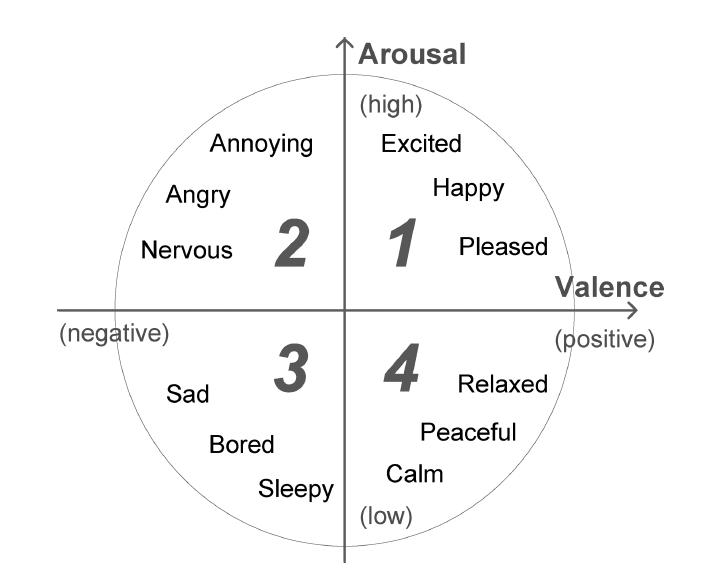
\includegraphics[width=0.9\textwidth]{russell.png}
        \legend{Fonte: \citeonline{russell1980circumplex}.}
\end{figure}

Nos estudos psicológicos os fatores utilizados no gráfico são \cite{osgood1957measurement} \cite{plutchik1980emotion}: 
\begin{itemize}
        \item 
            valência (agradabilidade ou estados afetivos positivos e negativos);
        \item 
            excitação (ativação, energia ou estimulação);
        \item 
            potência (domínio, senso de controle ou liberdade).
\end{itemize}

\citeonline{russell1980circumplex} propôs o modelo da figura \ref{fig_dim}, que consiste de um plano bidimensional, onde os eixos são valência e excitação, e assim como no círculo de Hevner (figura \ref{fig_hevner}), as emoções estão agrupadas e posicionadas de acordo com suas características e similaridades das emoções adjacentes.
Para embasar a organização e credibilidade da técnica de \citeonline{russell1980circumplex} foram escalados 28 termos afetivos de quatro maneiras diferentes: utilizando a técnica de \citeonline{ross1938statistic} para ordenar as variáveis de maneira circular, um procedimento de escala multidimensional baseado na similaridade dos termos, uma escala unidimensional hipotética de valência e excitação e a pesquisa com 343 indivíduos, onde os mesmos reportavam a maneira como estavam se sentindo \cite{russell1980circumplex}.

O modelo de representação dimensional representado na figura \ref{fig_dim} apresenta o ponto forte que é uma maneira simples de organizar as emoções de maneira robusta, mas \citeonline{lazarus1991emotion} levantaram questões sobre como a técnica obscurece importantes aspectos do processo emocional, como citado por \citeonline{yang2012machine} medo e raiva estão próximos conceitualmente, porém eles são bem diferentes quando observamos as reações físicas dos indivíduos. Tal questão incentivou a adição da potência \cite{bigand2005multidimensional}, formando assim um modelo tridimensional, porém o modelo se mostrou difícil de visualizar e acabou mostrando que em uma relação de complexidade e qualidade de definição de emoções, é preferível se trabalhar com o plano bidimensional\cite{juslin2001music}.
%%https://psycnet.apa.org/record/1981-25062-001
%%https://link.springer.com/chapter/10.1007/978-3-319-70609-2_9

Classificar músicas através das emoções é uma tarefa multidisciplinar que discretiza as emoções para que sejam processadas pelo computador. Cada representação tem como base um extenso trabalho de pesquisa \cite{kim2010music}. 

%% Talvez dar uma introdução a algumas características das músicas e ligar o estudo destas características com a definição da emoção da música, ligando diretamente a uma forma de definir a emoção de uma dada música a utilização do Aprendizado de Máquina
\subsection{Características Estruturais da Música}


\subsection{WIP - dificuldades da classificação de musicas por emoções}
O que é valencia?
O que é energia?
como são sintetizados?
por que o modelo de thayer e 

"almost every work differs in the way that it represents emotions. Similarly to psychological studies, there
is no real agreement on a common model." - Music Mood Representations from Social Tags

"But music itself is the expression of emotions, which can be highly subjective and difficult to quantify. Automatic recognition of emotions (or mood) in music is still in its early stages, though it has received increasing attention in recent years. Determining the emotional content of music audio computationally is, by nature, a crossdisciplinary endeavor spanning not only signal processing
and machine learning, but also requiring an understanding of auditory perception, psychology, and music theory" - MUSIC EMOTION RECOGNITION: A STATE OF THE ART REVIEW

\section{Aprendizado de máquina}
    % Escrever sobre aprendizado de maquina em si, pra n deixar uma subsection vazia
    
    % https://doi.org/10.1016/B978-0-08-051054-5.50005-4
    O aprendizado de máquina é um subcampo da ciência da computação que tem como objetivo otimizar a performance de algoritmos que, a partir de um dado e de uma respectiva base de dados que contém dados semelhantes, são caracterizados algoritmos preditivos, que tentam prever um dado futuro a partir da base de dados, ou de algoritmos descritivos, para obter mais conhecimento e novas informações a partir de um dado presente na base de dados\cite{alpaydin2009introduction}. 
    
    É chamado aprendizado de máquina porque em uma base de dados novos dados podem ser inseridos e o algoritmo deve ser organizado para aprender se adaptar com as mudanças da base de dados, fazendo com que o algoritmo tenha uma alta precisão preditiva\cite{alpaydin2009introduction}.
    
\subsection{K-Nearest Neighbors}
    No reconhecimento de padrões, o \textit{K-Nearest Neighbor} (KNN) é um algoritmo de classificação e aprendizado de máquina supervisionado não-probabilístico que utiliza uma função de distância para enumerar seus vizinhos mais próximos, assim definindo uma classe para um grupo de vizinhos\cite{5408784}.
    
    O KNN é baseado na distância Euclidiana entre o elemento teste que queremos classificar e os elementos já classificados. Calculada a distância euclidiana, assumimos os k elementos mais próximos do elemento teste e o classificamos com o conjunto dos elementos de maior ocorrência dentro destes k elementos. 
    
    A figura \ref{fig_knn} representa o funcionamento do algoritmo KNN, onde k = 4. No exemplo, o algoritmo calcula a distância euclidiana do novo elemento, representado por um quadrado verde na figura \ref{fig_knn}, para cada elemento do conjunto que já foi classificado e, a partir dos quatro itens mais próximos o elemento é classificado com a classe mais recorrente dos vizinhos, que no exemplo da figura \ref{fig_knn} é a Classe A (círculos vermelhos).
    
    \begin{figure}[ht]
        % http://scholar.google.com.br/scholar_url?url=http://scholarpedia.org/article/K-Nearest_Neighbor&hl=pt-BR&sa=X&scisig=AAGBfm3MB_Apy73InOnpDlzYaq23tyHBUA&nossl=1&oi=scholarr
        \advance\leftskip0.15\textwidth
        \caption{\label{fig_knn}Exemplo de classificação do algoritmo KNN}
        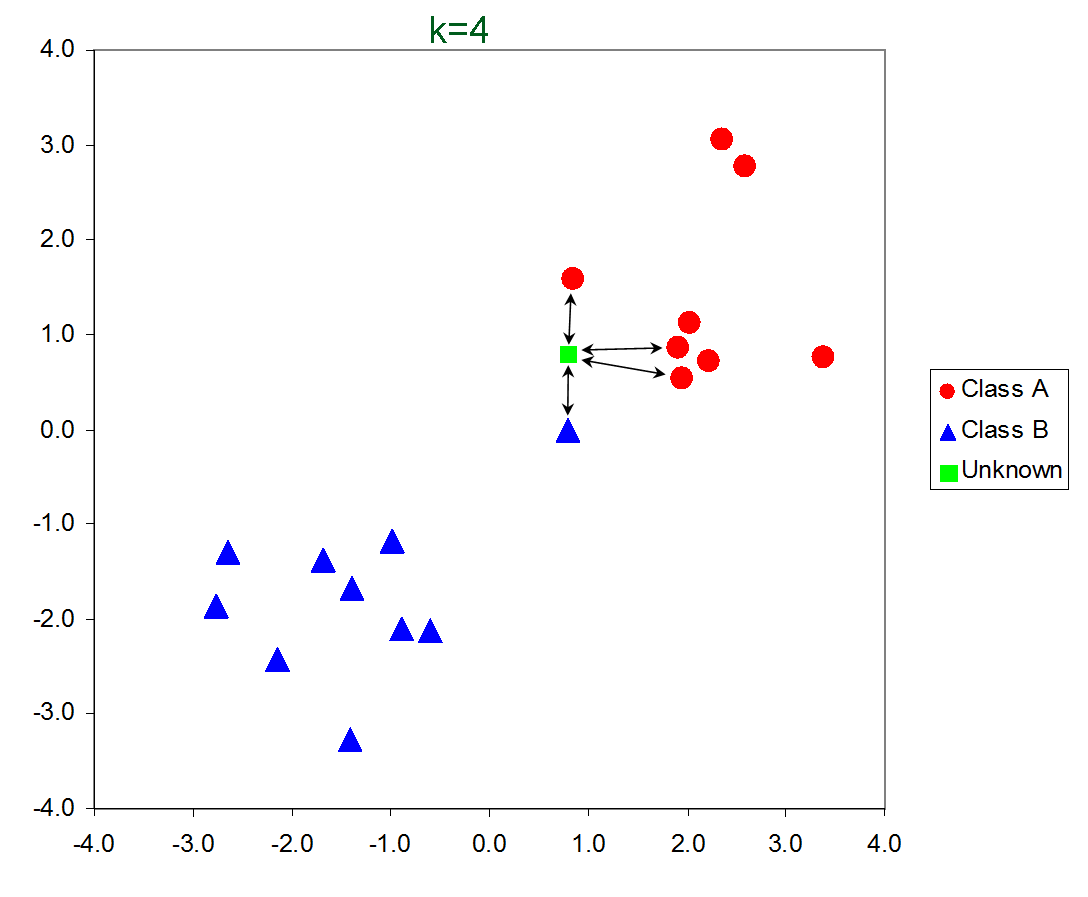
\includegraphics[width=0.8\textwidth]{knn.png}
        \legend{Fonte: \citeonline{leife.peterson2009}.}
    \end{figure}
\newpage
\subsection{Redes Neurais Artificiais}
    Redes Neurais Artificiais são modelos computacionais inspirados no sistema nervoso dos animais. No sistema nervoso temos células que chamamos de neurônios, tais estruturas por si só não possuem impacto significativo no sistema ou utilidade, porém o sistema nervoso contém  bilhões de neurônios \cite{lent2004cem}, todos eles se comunicando através de trocas química, formando assim uma rede neural. Assim formamos um sistema nervoso, que é um sistema complexo, através de conjuntos de neurônios, que são sistemas individualmente simples  \apudonline{lent2004cem}{leife.peterson2009}. 

    Nas redes neurais artificiais o neurônio é uma unidade lógica que pertence a uma camada da rede neural, sendo conectado através de sinapses com os neurônios da camada anterior e posterior, se existentes.
    
    É possível identificar três blocos blocos principais em uma Rede Neural Artificial \cite{ruano2003}:
    \begin{itemize}
        \item 
            Um conjunto de sinapses definidas por ligações entre os neurônios, que são associadas a pesos em uma matriz $W$, onde $W_{i,j}$, onde $i$ é o neurônio origem do sinal enviado através da sinapse e $j$ é o neurônio destino do sinal. Este peso é usado para multiplicar o sinal de entrada, que definirá o sinal de saída da sinapse;
        \item 
            Os sinais de entrada são integrados ao neurônio e existe um neurônio adicional, que serve como um neurônio somador ou simplesmente como outra entrada, com o valor fixo de 1;
        \item 
            Uma função de ativação ou de saída, onde o conjunto de saídas é $[0,1]$ ou $[-1,1]$, dependendo do método utilizado.
    \end{itemize}
    
    \begin{figure}[ht]
        % https://alok007.files.wordpress.com/2010/11/neural-networks.pdf
        \caption{\label{ann_example}Exemplo de rede neural artificial com uma camada de entrada e uma camada de saída}
        
        \begin{center}
            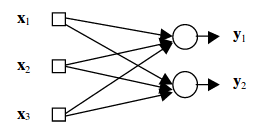
\includegraphics[]{single_layer_network.png}
        \end{center}
        
        \legend{Fonte: \citeonline{ruano2003}.}
    \end{figure}
    
    Na Figura 2, temos um exemplo de uma rede neural artificial com duas camadas: uma camada de entrada com 3 neurônios e uma camada de saída com 2 neurônios. Entre cada neurônio da camada de entrada e cada neurônio da camada de saída temos uma sinapse, cada uma com seu respectivo peso definido na matriz de pesos $W$.
    
\subsubsection{Multilayer Perceptron}
    % https://alok007.files.wordpress.com/2010/11/neural-networks.pdf
    O \textit{Multilayer Perceptron (MLP)} é uma rede neural multi-camada, onde existem $n$ camadas, sendo $L_0$ a camada de entrada, onde os dados são inseridos para o treinamento e, posteriormente, para a classificação, e $L_n$ a camada de saída, onde o neurônio com o maior valor de saída representa a classificação daquela entrada pelo algoritmo. As camadas intermediárias, chamadas de camadas ocultas, ligam todos os neurônios da sua camada aos neurônios das camadas anteriores e posteriores da rede através das sinapses, que têm pesos representados pela matriz $W$. Na Figura \ref{fig_mlp}, é possível observar as camadas detalhadamente de forma gráfica.

    \begin{figure}[H]
        % https://alok007.files.wordpress.com/2010/11/neural-networks.pdf
        \caption{\label{fig_mlp}Exemplo de esquematização de rede neural utilizado no MLP}
        
        \begin{center}
            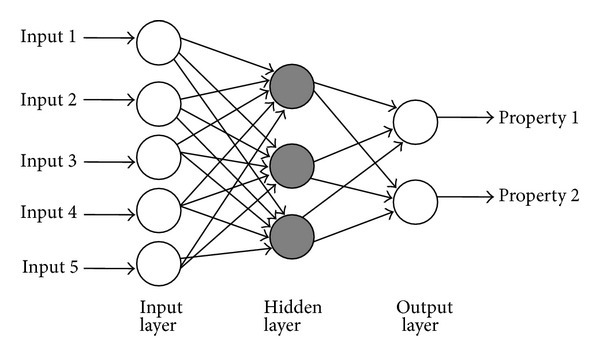
\includegraphics[width=0.7\textwidth]{mlp.png}
        \end{center}
        
        \legend{Fonte: \citeonline{jamesswarbrick2006}, p. 2400.}
    \end{figure}
    
    No MLP, a divisão do conjunto de dados é realizada em duas partes: o conjunto de treinamento e o conjunto de testes, sendo o conjunto de treinamento maior que o conjunto de testes, pois o treinamento da rede é fundamental neste algoritmo. 
    
    Durante o treinamento, as saídas esperadas pelo algoritmo no conjunto de dados já são conhecidas, tornando possível verificar a precisão da rede neural e obter o erro através da fórmula a seguir, onde $e_{obtido}$ é a saída obtida na rede neural e $e_{esperado}$ é a saída esperada, já existente no conjunto de dados.
    
    \[ e = e_{obtido} - e_{esperado}  \]

    O método utilizado para a atualização dos pesos da matriz de pesos $W$ no MLP é o algoritmo de \textit{Error Back-Propagation (BP)}. O BP propaga o erro obtido na saída da rede neural nos neurônios anteriores, até chegar à camada $L_0$, utilizando a fórmula gradiente na direção negativa da rede neural \cite{ruano2003}. A propagação do erro na direção inversa atualiza os pesos da rede neural, melhorando a precisão da classificação.

    Após o treinamento da rede neural, é executada a classificação pela rede utilizando o conjunto reservado para testes para definir a precisão final da rede neural.

\subsubsection{Rede Neural Convolucional}
    % Link de um livro pra CNN: https://books.google.com.br/books?id=EUhNDwAAQBAJ&printsec=frontcover&dq=Convolutional+Neural+Network&hl=pt-BR&sa=X&ved=0ahUKEwjUiLW20P7eAhVJOZAKHX2bC98Q6AEILjAB#v=onepage&q=Convolutional%20Neural%20Network&f=false
    % Capítulo 4, página 43, fala sobre CNN
    A Rede Neural Convolucional \textit{(CNN)} é uma categoria de rede neural utilizada para lidar com dados de alta dimensão, como vídeos e imagens. A \textit{CNN} funciona de forma muito similar à rede neural padrão, tendo como uma das diferenças a variação de tipos de camadas que processam os dados até ser possível realizar a sua classificação. \cite{salmankhanhosseinrahmanisyedafaqalishah2018}
    
    Segundo \citeonline{salmankhanhosseinrahmanisyedafaqalishah2018}, as diversas camadas da \textit{CNN} podem implementar algumas funcionalidades básicas, como as camadas de convolução, agregação, centralização e as camadas totalmente conectadas, ou até algumas funcionalidades mais complexas, como a \textit{Spatial Transformer Layer} e a \textit{VLAD Pooling Layer}.
    
    Segundo \citeonline{salmankhanhosseinrahmanisyedafaqalishah2018}, são definidas como camadas específicas da \textit{CNN} o pré-processamento dos dados. São alguns dos métodos que podem ser utilizados nesta camada:
    \begin{itemize}
        \item 
        O método da subtração média, onde os valores da entrada são subtraídos pela média calculada no conjunto de treinamento, definindo o peso como $x' = x - \hat{x}$, onde $\hat{x}$ é definido por $\frac{1}{N} \sum_{i=1}^{N} x_i$;
        
        \item
        O método da normalização, onde os pesos de entrada são divididos pelo desvio padrão de cada dimensão dos valores de entrada.
    \end{itemize} 
    
    A camada de convolução contém um conjunto de filtros, que consistem numa matriz com números discretos denominados pesos. Estes pesos são atualizados a cada iteração da \textit{CNN} e são multiplicados com os valores de entrada desta camada, gerando assim um mapa que consiste na convolução dos valores de entrada com o filtro. É possível ver um exemplo do funcionamento dessa camada na Figura \ref{fig_cnn_conv}. Pode ser utilizado para a realização desta convolução:
    \begin{itemize}
        \item 
        O método da convolução válida, onde não é necessário ter o deslocamento da matriz de entrada. Neste método, se a matriz de entrada tem tamanho 4x4, a matriz resultante terá tamanho 3x3;
        
        \item
        O método da convolução igualitária, que garante que a matriz de entrada da camada e a matriz resultante da convolução tenham o mesmo tamanho. Para chegarmos a um resultado que satisfaça essa igualdade, a matriz de entrada é deslocado. Também é chamada de "meia convolução";
        
        \item
        O método da convolução completa, que consiste na aplicação do deslocamento máximo na matriz de entrada a fim de ter pelo menos um valor da entrada presente em todas as multiplicações feitas pelo filtro.
    \end{itemize} 
    
    \newpage
    
    \begin{figure}[ht]
        \caption{\label{fig_cnn_conv}Exemplo do que acontece na camada de convolução}
        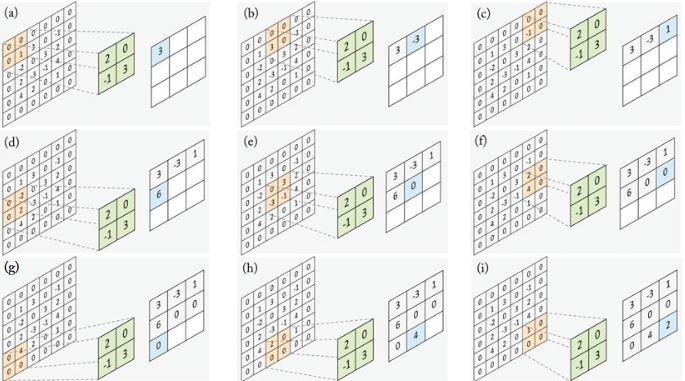
\includegraphics[width=\textwidth]{CNN-ConvLayer.JPG}
        \legend{Fonte: \citeonline{salmankhanhosseinrahmanisyedafaqalishah2018}.}
    \end{figure}
    
    %Pooling
    A camada de agregação consiste na aplicação de uma operação combinatória em uma região matricial de tamanho predefinido, com o movimento dessa região em um passo predefinido. A operação de combinação pode ser o cálculo do valor máximo da região matricial ou a média dos valores que a matriz contém. Se o tamanho da região da combinação for definida por $f x f$, com o tamanho do passo $s$, o novo tamanho da matriz é definido por
        $$h' = \left \lfloor{\frac{h - f + s}{s}} \right \rfloor,   w' = \left \lfloor{\frac{w - f + s}{s}} \right \rfloor$$
    onde h' é a altura nova e w' é a largura nova da matriz.
    
    É possível ver um exemplo do funcionamento dessa camada na Figura \ref{fig_cnn_pool}.
    \begin{figure}[H]
        \caption{\label{fig_cnn_pool}Exemplo do que acontece na camada de agregação}
        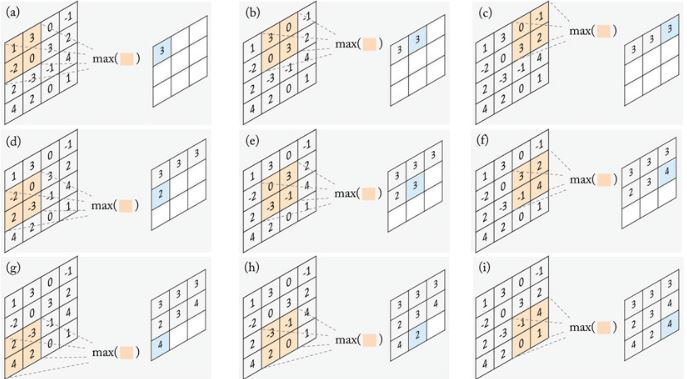
\includegraphics[width=\textwidth]{CNN-PoolingLayer.JPG}
        \legend{Fonte: \citeonline{salmankhanhosseinrahmanisyedafaqalishah2018}.}
    \end{figure}
    
    Com a imagem representada pela matriz de entrada, temos a execução do pré-processamento da imagem através das camadas iniciais e o processamento da matriz resultante processada nas várias camadas de convolução e agregação para que o tamanho da matriz seja filtrado até um tamanho onde pode ser realizada a classificação da imagem, como podemos ver na Figura \ref{fig_cnn_example}.
    
    \begin{figure}[ht]
        \caption{\label{fig_cnn_example}Exemplo de aprendizado supervisionado para classificação de imagens}
        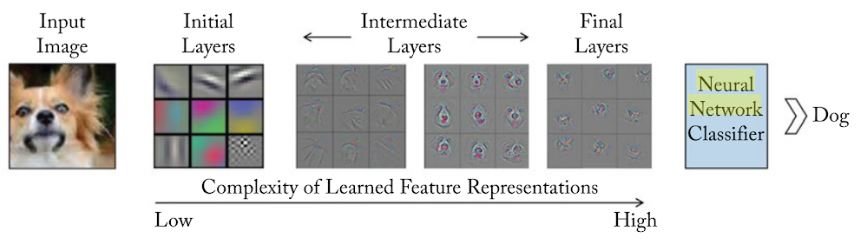
\includegraphics[width=\textwidth]{CNN.JPG}
        \legend{Fonte: \citeonline{salmankhanhosseinrahmanisyedafaqalishah2018}.}
    \end{figure}
\newpage
\section{Trabalhos Relacionados}
    Nesta Seção serão tratados trabalhos relevantes da área de pesquisa do presente trabalho de conclusão de curso, para classificação de músicas quanto as supostas emoções provocadas pelas mesmas. O trabalho \textit{Comparison between Weighted D-KNN and Other Classifiers for Music Emotion Recognition} compara uma técnica derivada do \textit{KNN} a técnicas comumente utilizadas para o reconhecimento de emoções contidas numa música e o trabalho \textit{Music Mood Detection Based on Audio and Lyrics with Deep Neural Net} utiliza dados da letra da música e alguns dados sobre o próprio áudio de forma multimodular, ou seja, combinando o resultado dos dois processamentos, para detectar o sentimento causado pela música.
    
    % Palavras Chave: Música, Emoção, KNN, Classificação
    
    % Periodo de busca para técnicas e algoritmos entre 2000 e até o momento, uma vez que \citeonline{yang2012machine}, comenta que a busca por esse tipo de classificação se intensificou com o consumo de midias através de computadores e mp3. já a parte filosófica e psicológica, com inicio por volta de 1950 até atualmente.
    
    % Nesta Seção serão tratados trabalhos, métodos e técnicas para detecção e discriminação de plantas, classificando-as como ervas daninhas ou outro tipo de planta. O trabalho \textit{Weed-Plant Discrimination By Machine Vision and Artificial Neural Network} possui ênfase em pre-processar as imagens com programas de edição de imagem, para discretizar as informações das plantas e classifica-las utilizando uma rede neural artificial e o trabalho \textit{Weed and crop discrimination using image analysis and artificial intelligence methods} utiliza visão computacional em conjunto com uma Rede Neural Auto-Associativa, com alguns ambientes de controle para treinamento, para diferenciar uma plantação de cenouras de ervas daninhas.
 
    
    \subsection{Comparison between Weighted D-KNN and Other Classifiers for Music Emotion Recognition}
        Em \textit{Comparison between Weighted D-KNN and Other Classifiers for Music Emotion Recognition} \cite{Pao2008}, é proposto o desenvolvimento de uma técnica de classificação das músicas utilizando a técnica variante do KNN chamada Weighted D-KNN, que consiste numa versão que utiliza pesos que otimizam a acurácia da classificação. É feita uma comparação do desempenho do Weighted D-KNN com o desempenho de outros classificadores populares, que são o KNN e o SVM, aplicando-os a um banco de dados de músicas composto por 60 famosas canções populares de álbuns ingleses. As emoções das músicas foram classificadas por 40 participantes. 

        Para representação das emoções foi utilizado a representação dimensional de \citeonline{russell1980circumplex}, e para extração dos dados das músicas foram utilizadas as aplicações PsySound e Maryas.

        Os resultados experimentais mostram que a proposta do classificador W-D-KNN alcança uma taxa de reconhecimento maior que 96\% e supera o KNN e o SVM.
    %acho que agora só falta consertar o começo dos trabalhos relacionados
    % bele
    % Já volto ok
    %Trabalho da Deezer
    \subsection{Music Mood Detection Based on Audio and Lyrics with Deep Neural Net}
        \textit{Music Mood Detection Based on Audio and Lyrics with Deep Neural Net} \cite{DBLP:journals/corr/abs-1809-07276} tem o objetivo de detectar a emoção musical a partir de dois módulos diferentes: as letras e o próprio áudio da música. Neste trabalho são utilizadas técnicas de \textit{Deep Learning}, como Redes Neurais Convolucionais, e uma base de dados com 18 mil músicas descritas com seus níveis de excitação e valência, construída com base no \textit{Million Song Dataset}\cite{Bertin-mahieux11themillion} e no catálogo do Deezer.
    
        O autor indica que a emoção na música deve ser estudada de forma multimodular, analisando tanto o áudio da música quanto as letras, pois estes são processados por áreas diferentes do cérebro humano.
    
        \begin{figure}[ht]
            \caption{\label{fig_deezer_multimodal}Arquitetura dos modelos unimodulares e multimodular}
            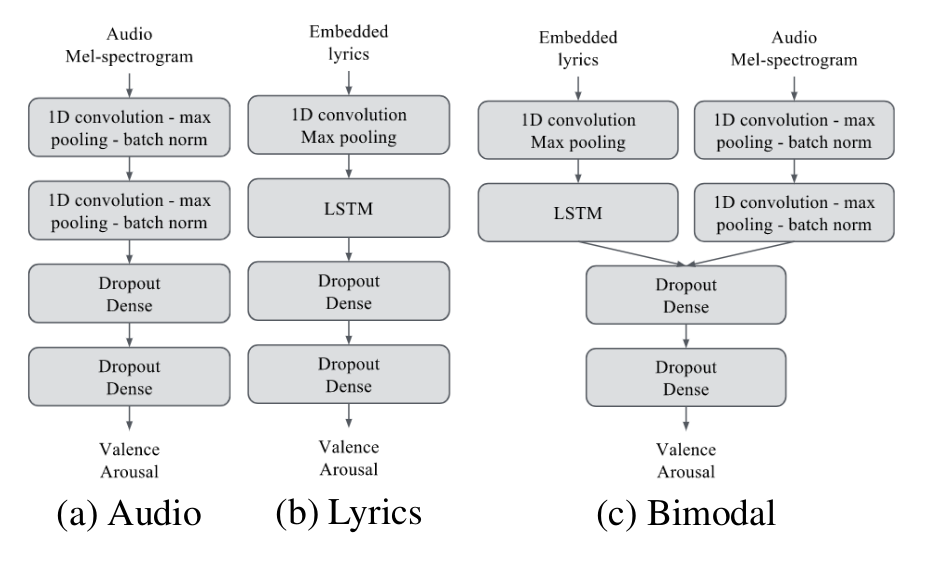
\includegraphics[width=\textwidth]{Deezer_MultiModal_Architecture.png}
            \legend{Fonte: \citeonline{DBLP:journals/corr/abs-1809-07276}.}
        \end{figure}
    
        Na figura \ref{fig_deezer_multimodal}, podemos observar como os módulos de áudio e letra são representados individualmente utilizando CNN e como o modelo multimodular concatena as saídas das redes neurais tanto de áudio quanto de letra para dar uma saída mais precisa e embasada sobre a emoção passada música. Este embasamento acaba sendo abrangente na questão cultural da música, pois mostra como a música pode ser interpretada por nativos da língua da música (áudio e letra) e por pessoas que só estão interessadas no ritmo e na melodia (áudio).
    
        Este trabalho conclui que a detecção de excitação e valência de uma música utilizando a metodologia de \textit{Deep Learning} e uma abordagem multimodular alcança melhores resultados do que as aproximações clássicas utilizadas para tal.

\chapter[Desenvolvimento]{Desenvolvimento}
% Proposta
% Como medir o resultado
    Para o desenvolvimento do Trabalho de Conclusão de Curso, será aplicada uma técnica de aprendizado de máquina para classificar a música quanto suas emoções transmitidas, utilizando tanto dados sobre o áudio da música obtidos pela API do Spotify quanto a letra da música, que é obtida por uma biblioteca do Python. 
    
    O conjunto de emoções a ser utilizado será o definido por \cite{russell1980circumplex}, onde existem 28 emoções que tem intensidades diferentes de cada uma das emoções descritas na representação gráfica de valência e agitação mostrada pela Figura \ref{fig_dim}. As 28 emoções e as intensidades das 8 emoções distribuídas na representação da Figura \ref{fig_dim} estão representadas na Figura \ref{fig_emotion_table}.
    
    \begin{figure}[H]
        \caption{\label{fig_emotion_table} Representação em tabela .}
        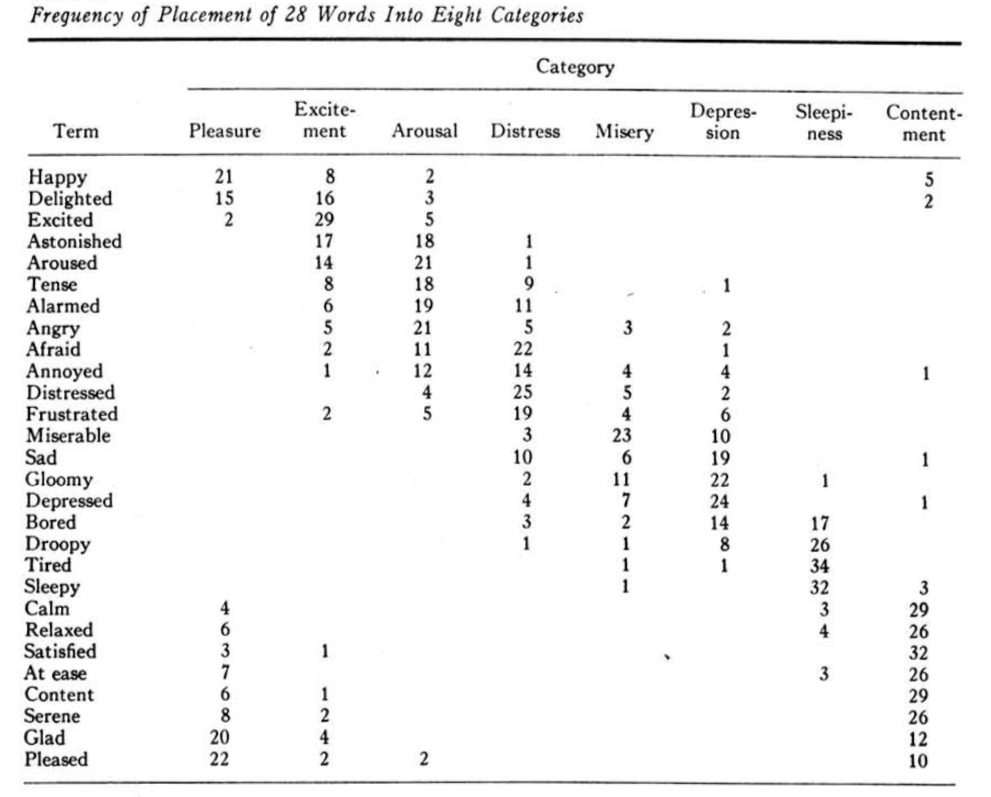
\includegraphics[width=\textwidth]{3DC01B5E-5237-4172-8E7D-3200AB0E0026.jpeg}
        \legend{Fonte: \citeonline{russell1980circumplex}.}
    \end{figure}
    
    Utilizando o conjunto de dados do Million Song Dataset, é possível obter um conjunto de músicas genérico que pode atender uma quantidade maior de pessoas, com músicas mais variadas. Desta forma, na etapa de validação dos resultados, será obtido um conjunto de músicas relacionado a um conjunto maior de emoções, pois sua variedade rítmica é mais abrangente.
    
    Utilizando a API do Spotify é possível conhecer alguns dados técnicos sobre a música, como mostra o exemplo da Figura \ref{fig_spotify_api}. 
    
    \begin{figure}[H]
        \caption{\label{fig_spotify_api}Exemplo de retorno da API do Spotify}
        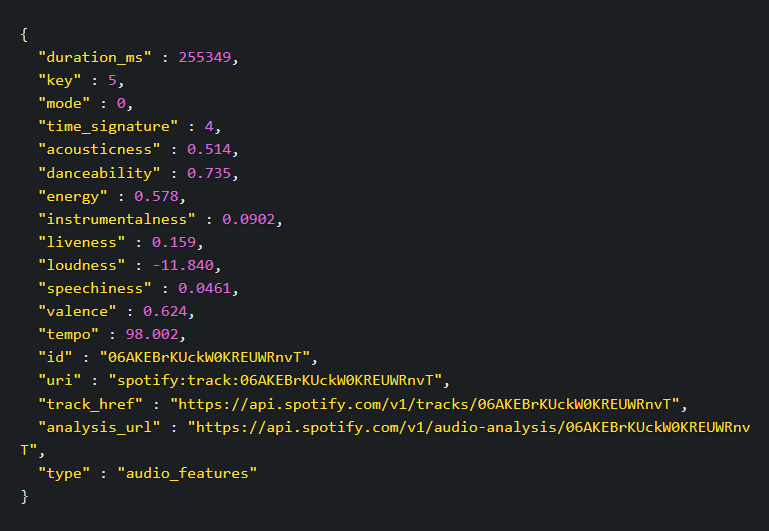
\includegraphics[width=\textwidth]{SpotifyAPI.PNG}
        \legend{Fonte: Documentação da API do \citeonline{spotifyapi}.}
    \end{figure}
    
    Alguns atributos importantes presentes nestes dados técnicos que têm seu valor variando entre 0.0, que significa a ausência do atributo, e 1.0, que identifica a totalidade do atributo, são \textit{acousticness}, que determina a confiabilidade de que a música é acústica, \textit{danceability}, que representa como o tempo, a estabilidade do ritmo e a força da batida contribuem para que a música seja mais dançante, \textit{energy}, que mostra quão enérgica e intensa é a música, \textit{instrumentalness}, que define se a música é composta somente de instrumentos ou não, \textit{liveness}, que identifica se há uma audiência na gravação, indicando que a música é gravada ao vivo, \textit{valence}, que indica a positividade e alegria da música, onde quanto maior é o valor mais alegre é a música. Também há alguns outros atributos que interferem diretamente nas características emocionais da música, como \textit{tempo} (batidas por minuto), variando entre 0 e 250 BPM, e \textit{loudness}, que sinaliza o volume médio da música em decibéis, variando tipicamente entre -60 e 0 decibéis.
    
    Obtendo os dados da API do Spotify, as emoções da música serão definidas através do \textit{KNN}; já para os dados da letra da música, será aplicado o cálculo dos termos mais relevantes da letra utilizando o valor \textit{TF-IDF} e, a partir destes valores relacionados aos termos da letra, serão utilizadas técnicas de rede neural para definir as palavras mais comuns relacionadas ao conjunto de emoções definidos, classificando assim a música em suas respectivas emoções transmitidas.
    
    A multimodularização utilizando dados do áudio e do texto será essencial pois, segundo \citeonline{DBLP:journals/corr/abs-1809-07276}, uma abordagem multimodular alcança melhores resultados, além de garantir o resultado médio considerando a semântica e o ritmo, o que possibilita descrever a emoção transmitida pela música independente do ouvinte conhecer ou não o idioma. 
    
    Será utilizado a técnica \textit{KNN} para classificar a música a partir dos dados obtidos através da API do Spotify pela performance e a simplicidade do algoritmo, pois será calculado através de dados já processados de forma contínua pelo Spotify, tornando assim o agrupamento dentro das emoções definidas por \citeonline{russell1980circumplex} mais simples e rápido. 
    
    Utilizando a biblioteca lyricsgenius do Python é possível receber a letra da música e, a partir do cálculo dos valores \textit{TF-IDF} para cada termo, serão extraídas as palavras mais relevantes da letra da música. Esta letra será passada para uma rede neural, processando as palavras e classificando as emoções que esta música transmite.
    
    A validação dos resultados será feita a partir da metodologia de Survey, ao construir um Termo de Consentimento Livre e Esclarecido (TCLE) para trazer confiabilidade à pesquisa. Será apresentado um subconjunto das músicas já processadas com suas emoções já calculadas para um conjunto de no máximo 10 não músicos, pois segundo \citeonline{sloboda2001daily}  os não músicos têm uma percepção técnica menos aprimorada que músicos acerca das emoções que a música pode proporcionar. Com isto, será possível determinar a assertividade das técnicas utilizadas, definindo se as emoções definidas sobre a música coincidem com as emoções descritas pelo usuário. 


% ----------------------------------------------------------
% ELEMENTOS PÓS-TEXTUAIS
% ----------------------------------------------------------
\postextual
% ----------------------------------------------------------

% ----------------------------------------------------------
% Referências
% ----------------------------------------------------------
\bibliography{ref}{}
\bibliographystyle{abntex2-alf}


\end{document}